\section{Motor med tilh. H-bro på bil}

Motorkredsløbet for AU2 vil potentielt være et større EMC-problem, da en højfrekvent og stor strøm løber igennem dele af kredsløbet.
Da motoren drives af et relativt højfrekvent PWM signal, hvis flanker går fra stel til forsyning (7.2V) og der iøvrigt trækkes relativt store strømme. 
Ydermere forventes et spændingspeak når motoren afbrydes ved hver periode, da der løber strøm i spolen og denne strøm ingen steder kan løbe umiddelbart.
Dette giver anledning til højere harmoniske frekvenser af grundfrekvensen i PWM signalet og det vurderes derved at motor agerer som en kraftig støjkilde.

\begin{figure}[h]
\centering
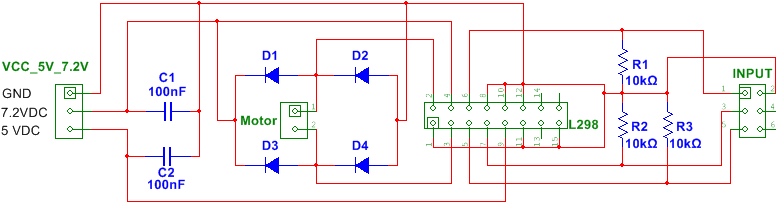
\includegraphics[width=\textwidth]{../fig/billeder/hbro_multisim.png}
\caption{Design af motorens Hbro i Multisim.}
\label{fig:hbro_multisim}
\end{figure}
 
For at modvirke dette er der placeret en kondensator parallelt med motoren, som derved fjerner en stor del af den højfrekvente støj som opstår. 
OBS: Denne kondensator fremgår ikke af figur \ref{fig:hbro_multisim}. 
Dog vil strømmen der tænder og slukker i ledningerne før motoren, kunne give problemer ifm. nærværende ledninger/printbaner. 

\begin{figure}[h]
\centering
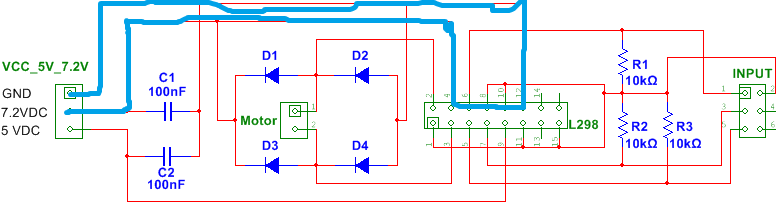
\includegraphics[width=\textwidth]{../fig/billeder/hbro_multisim_loop.png}
\caption{Design af motorens Hbro i Multisim.}
\label{fig:hbro_multisim_loops}
\end{figure}

De strømloops der er i H-broen kan ses på figur \ref{fig:hbro_multisim_loops}. Det blå loop er den strøm der løber fra kondensatoren C1 gennem H-broen til motoren og tilbage via stel. C1 har desuden til formål at reducere støj fra motorkredsløbet på forsyningsnettet.
Det grønne loop er den vej strømmen løber, når enable signalet til H-broen netop er frakoblet og motoren vil forsøge at aflevere energi tilbage til C1. Den forhindrer således spændingspeak fra motoren, men resultatet bliver et strømloop som støjer. Det grønne loop har et tilsvarende strømloop gennem D3 og D2, når DC-motoren kører modsatrettet.
Printet til motorkredsløbet er forsøgt designet således, at de strømloops der er, konstrueres så små som mulige og at banerne med stor risiko for støj er placeret så langt som muligt fra andre baner. Desuden er der placeret et Ground plan, der foruden at forøge stelkapaciteten gør det nemmere for højfrekvente strømme, at finde den returvej med mindst modstand. Printudlægget kan ses på figur \ref{fig:hbro_ultiboard}.
C1 og C2 er placeret på bagsiden af printet under D2, dette kan godt være svært at se grundet farvevalget.

Som en ekstra forsikring mod common-modestøj, kan man med tilledningerne ud til motoren påsætte en ferritkerne omkring, som derved vil fjerne meget af støjen fra den strøm som løber ud til motoren.

\begin{figure}[h]
\centering
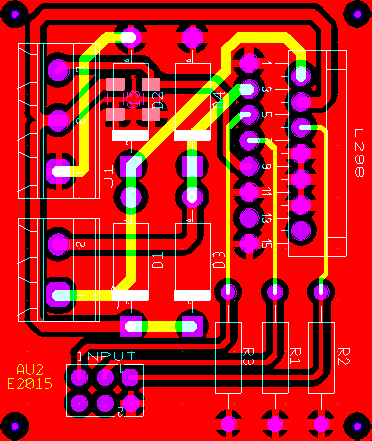
\includegraphics[scale=1]{../fig/billeder/hbro_ultiboard.png}
\caption{Printdesign af motorens Hbro i Ultiboard.}
\label{fig:hbro_ultiboard}
\end{figure}

